\subsection{OPTICS}
We have tested on each dataset 9 different configurations of the OPTICS algorithm, by using the 3 different
distance metrics (euclidean, manhattan and chebyshev) with 3 different the algorithms for nearest-neighbor search
 during the clustering process. Unlike many algorithms we will see next, OPTICS is deterministic, so it only needs to be run once.
\subsubsection{Hyperparameter Study}
For the different datasets, appropriate values for the hyperparameters were selected. The values used are presented in Table \ref{tab:optics}.
\begin{table}[h!]
    \centering
    \begin{tabular}{|c|c|c|c|}
    \hline
    Hyperparameter     & Hepatitis & Mushroom & Pen-based \\ \hline
    xi                 &  0.05         &   0.1       &  0.02         \\ \hline
    min\_samples       &     5      &     10     &     10   \\ \hline
    min\_cluster\_size &     0.05      &     0.1     &    0.05       \\ \hline
    \end{tabular}
    \end{table}
\subsubsection{Best runs}


\begin{table}[h!]
	\centering
	\begin{tabular}{|c|c|c|c|c|c|c|c|c|c|c|c|c|}
		\hline
		& \multicolumn{3}{c|}{Hepatitis} & \multicolumn{3}{c|}{Mushroom} & \multicolumn{3}{c|}{Pen-Based} \\ \hline
		Metric & \textit{d} & \textit{Algorithm} & \textit{Value} & \textit{d} & \textit{Algorithm} & \textit{Value} & \textit{d} & \textit{Algorithm} & \textit{Value} \\ \hline
		ARI            & -          & -         & 0  & chebyshev & brute & 0.8251         & euclidean & brute & 0.9990 \\ \hline
		NMI            & -          & -         & 0  & chebyshev & brute & 0.7643         & euclidean & brute & 0.9973 \\ \hline
		DBI            & euclidean  & brute     & 0.5574   & chebyshev & brute & 0.7103         & manhattan & brute & 0.7329 \\ \hline
		Silhouette     & euclidean  & brute     & 0.6425   & chebyshev & brute & 0.5041         & euclidean & brute & 0.5312 \\ \hline
		CHS            & euclidean  & brute     & 54.8359  & chebyshev & brute & 4530           & chebyshev & brute & 3688 \\ \hline
	\end{tabular}
	\caption{Best configurations and their corresponding parameter values (\texttt{n\_clusters}, \textit{m}, \(\rho\)) and metric values for sg-FCM across the three datasets.}
	\label{tab:optics_best_runs}
\end{table}



\begin{figure}[H]
	\centering
	\begin{subfigure}{0.32\textwidth}
		\centering
		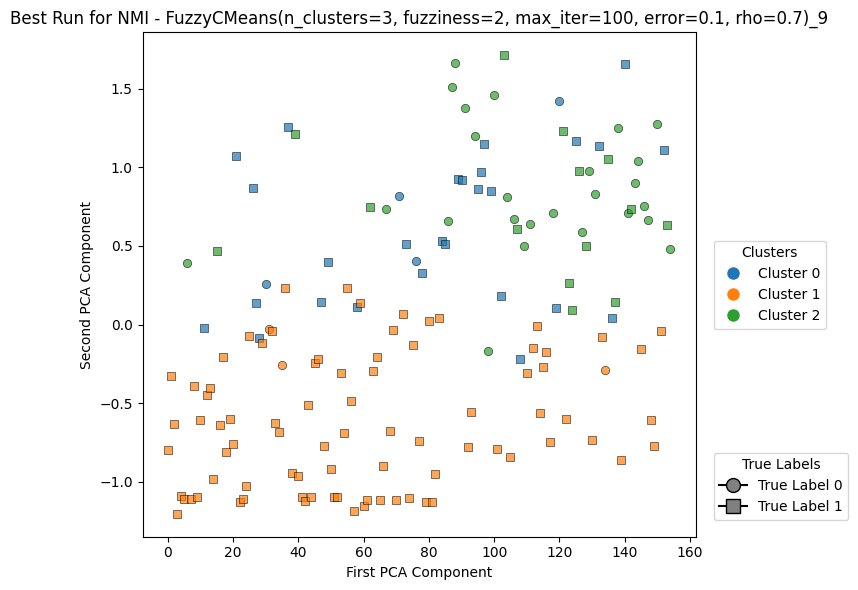
\includegraphics[width=\linewidth]{figures/FuzzyCMeans/Hepatitis/best_run_NMI.png}
		\caption{Hepatitis Dataset (NMI)}
	\end{subfigure}
	\hfill
	\begin{subfigure}{0.32\textwidth}
		\centering
		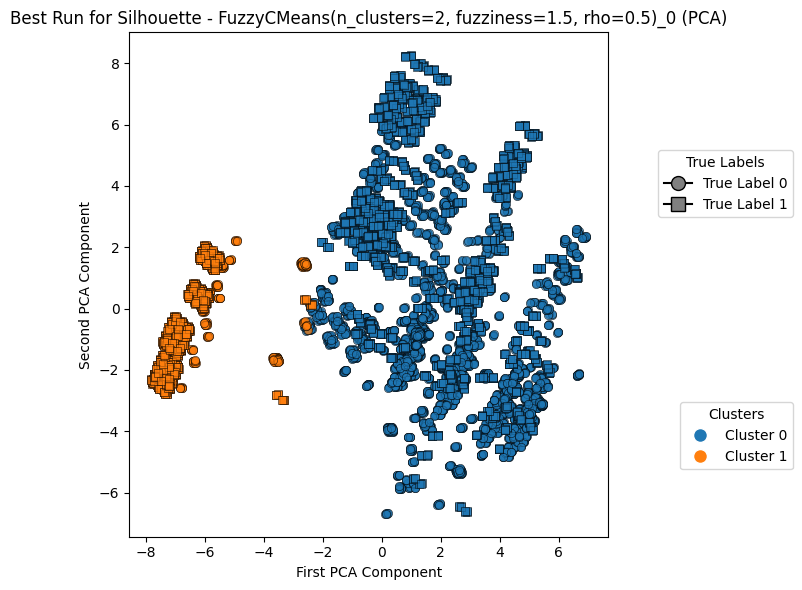
\includegraphics[width=\linewidth]{figures/FuzzyCMeans/Mushroom/best_run_Silhouette.png}
		\caption{Mushroom Dataset (CHS)}
	\end{subfigure}
	\hfill
	\begin{subfigure}{0.32\textwidth}
		\centering
		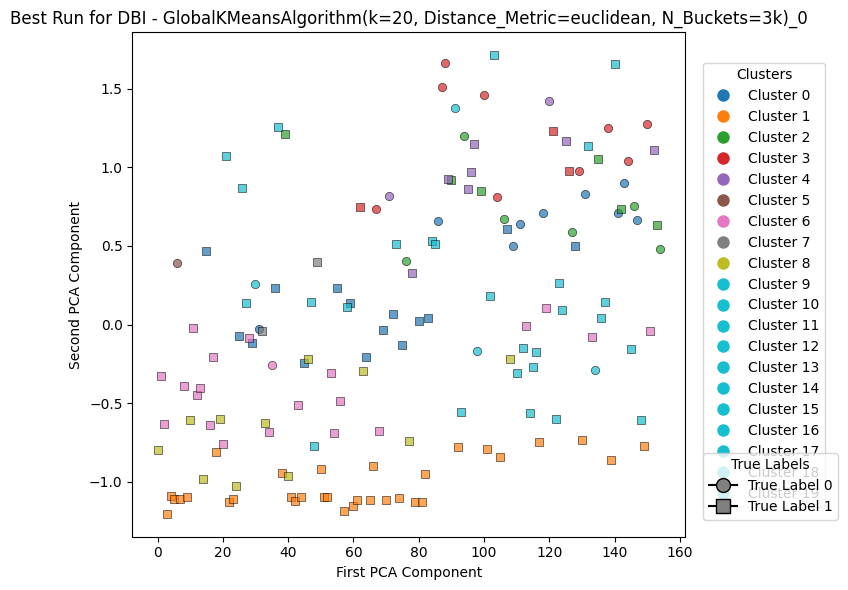
\includegraphics[width=\linewidth]{figures/FuzzyCMeans/PenBased/best_run_DBI.png}
		\caption{Pen-Based Dataset (Silhouette)}
	\end{subfigure}
	\caption{Resulting clusters for each dataset using the best sg-FCM configurations (after PCA).}
	\label{fig:sgfcm:clusters}
\end{figure}